\documentclass[english,brazil]{dissertacaoudesc}
\usepackage{graphicx}  % Permite mostrar imagens


% Informações do Aluno

\autor{Nome do Aluno}


% Informações do Orientador

% Descomente a linha a seguir para mudar o rótulo "Orientador:"
%\orientadorrotulo{Orientadora}
% Descomente a linha a seguir para mudar o título do orientador
%\orientadortitulo{Prof. Dra.}
\orientador{Nome do Orientador}
\orientadorinstituicao{UDESC}


% Informações do Coorientador

%\coorientadorrotulo{Coorientadora}
%\coorientadortitulo{Prof. Dra.}
% Descomente as linhas a seguir caso o trabalho tenha um coorientador
%\coorientador{Nome do Coorientador}
%\coorientadorinstituicao{UDESC}


% Informações da Instituição

\instituicao{Universidade do Estado de Santa Catarina}
\instituicaosigla{UDESC}
\centro{Centro de Ciências Tecnológicas}
\centrosigla{CCT}
\curso{Mestrado Acadêmico em Computação Aplicada}
\tipotrabalho{Dissertação}
\local{Joinville}


% Informações do Trabalho

\titulo{Título do Trabalho}
%\subtitulo{Subtítulo do Trabalho}
%\volume{1}
\datacompleta{xx de xx de 2020}
\data{2020}
\palavraschave{Latex. Abntex. Editoração de texto.}
\keywords{Latex. Abntex. Text editoration.}
\preambulo{Dissertação apresentada ao Programa de Pós-Graduação em Computação Aplicada, da Universidade do Estado de Santa Catarina, como requisito parcial para obtenção do grau de Mestre em Computação Aplicada.}


% Metadados do PDF

\hypersetup{
    pdfauthor=\imprimirautor,
    pdftitle=\imprimirtitulo,
    pdfkeywords=\imprimirpalavraschave,
    pdfsubject=\imprimirpreambulo,
}


% Conteúdo

\begin{document}
    \capa


    % Elementos Pré-textuais

    \imprimirfolhaderosto*

    \begin{fichacatalografica}
        % Siga as intruções em <https://www.udesc.br/bu/manuais/ficha> e a inclua com o comando a baixo
        %\includepdf{ficha_catalografica.pdf}
        % Ou utilize o exemplo a seguir:
        \begin{fichacatalograficaexemplo}
            1. Tópico 01.
            2. Tópico 02.
            I. \imprimirorientadortitulo~\imprimirorientador.
            II. \imprimirinstituicao.
            III. \imprimircentro.
            IV. identificação xxxx.
        \end{fichacatalograficaexemplo}
    \end{fichacatalografica}

    \begin{folhadeaprovacao}
        \begin{folhadeaprovacaoexemplo}
            Dr. Nome Completo 1 \\ UDESC
            \vspace{2\onelineskip}

            Dr. Nome Completo 2 \\ UDESC
            \vspace{2\onelineskip}

            Dr. Nome Completo 3 \\ UDESC
        \end{folhadeaprovacaoexemplo}
    \end{folhadeaprovacao}

    \begin{dedicatoria}
    Dedico este trabalho aos meus familiares, amigos, colegas e professores que me acompanharam e me deram forças nessa magnífica trajetória.
\end{dedicatoria}

    \begin{agradecimentos}
    Escreva seus agradecimentos aqui...
\end{agradecimentos}

    \begin{resumo}
    Lorem ipsum dolor sit amet, consectetur adipiscing elit. Morbi sit amet dolor ut eros tincidunt consequat vitae vitae quam. Vestibulum molestie id elit interdum rhoncus. Aenean aliquet dolor in lorem dictum, sit amet cursus tortor viverra. Nam suscipit molestie leo quis lobortis. Donec sit amet felis at magna fringilla pretium ut a purus. Donec placerat, augue id aliquet rhoncus, purus ante ullamcorper felis, ac luctus urna neque in velit. Quisque porta ex sit amet porttitor imperdiet. Donec auctor feugiat tellus ac elementum. Nulla non magna id risus volutpat cursus. Nullam semper, lectus et ultricies rutrum, lacus magna porttitor neque, venenatis aliquet metus odio vel justo. In lorem orci, dapibus ut est vitae, pharetra pharetra diam. Nulla luctus vestibulum convallis. Integer nec ipsum nibh.
\end{resumo}

    \begin{resumoingles}
    Lorem ipsum dolor sit amet, consectetur adipiscing elit. Morbi sit amet dolor ut eros tincidunt consequat vitae vitae quam. Vestibulum molestie id elit interdum rhoncus. Aenean aliquet dolor in lorem dictum, sit amet cursus tortor viverra. Nam suscipit molestie leo quis lobortis. Donec sit amet felis at magna fringilla pretium ut a purus. Donec placerat, augue id aliquet rhoncus, purus ante ullamcorper felis, ac luctus urna neque in velit. Quisque porta ex sit amet porttitor imperdiet. Donec auctor feugiat tellus ac elementum. Nulla non magna id risus volutpat cursus. Nullam semper, lectus et ultricies rutrum, lacus magna porttitor neque, venenatis aliquet metus odio vel justo. In lorem orci, dapibus ut est vitae, pharetra pharetra diam. Nulla luctus vestibulum convallis. Integer nec ipsum nibh.
\end{resumoingles}

    \imprimirlistadefiguras
    \imprimirlistadetabelas
    \begin{siglas}
    \acro{OV}{Organização Virtual}
    \acrodefplural{OV}{Organizações Virtuais}
    \acro{SDN}{\textit{Software Defined Networking}}
    \acro{SGBD}{Sistema de Gerenciamento de Banco de Dados}
\end{siglas}

    \begin{simbolos}
    \item[\%] Porcentagem
    \item[$D_{ab}$] Distância Euclidiana
    \item[$O(n)$] Ordem de um algoritmo
\end{simbolos}

    \imprimirsumario


    % Elementos Textuais

    \textual

    \chapter{Exemplo}\label{texto:exemplo}

Este capítulo é um exemplo de utilização deste template, apresentando como utilizar os elementos oferecidos.

Para mais informações veja a documentação dos pacotes:

\begin{incisos}
    \item \url{https://www.ctan.org/pkg/memoir}
    \item \url{https://www.ctan.org/pkg/abntex2}
\end{incisos}

\section{Citação}\label{texto:exemplo:citacao}

\subsection{Citação curta}\label{texto:exemplo:citacao:curta}

A citação curta vai no decorrer do texto entre aspas, como ``exemplo de citação curta'' \cite[p.~20]{exemplodelivro}. Ou como citação indireta por \citeonline{exemplodelivro}.

Resumidamente, utilize:

\begin{verbatim}
    \cite{exemplodelivro}  ->  (AUTOR, 2020)
    \cite[p.~20]{exemplodelivro}  ->  (AUTOR, 2020, p. 20)
    \citeonline{exemplodelivro}  ->  AUTOR (2020)
\end{verbatim}

\subsection{Citação longa}\label{texto:exemplo:citacao:longa}

\begin{citacao}
    Exemplo de citação longa, transcrevendo o texto dentro de um contexto \texttt{citacao} do Latex \cite[p.~20-21]{exemplodelivro}.
\end{citacao}

Ela também pode ser feita em inglês:

\begin{citacao}[english]
    Text in English language in italic with correct hyphenation \cite[p.~20]{exemplodelivro}.
\end{citacao}

\subsection{Apud}\label{texto:exemplo:citacao:apud}

Este é um exemplo de apud: \apud{exemplodelivro}{exemplodeartigo}, ou \apudonline{exemplodelivro}{exemplodeproceedings}.

\section{Texto em inglês}\label{texto:exemplo:textoingles}

\begin{otherlanguage*}{english}
    English text that can automatically receive hyphens if needed.
\end{otherlanguage*}

\section{Figura}\label{texto:exemplo:figura}

A \autoref{fig:grafico} mostra um gráfico, que também pode estar lado a lado com outro, como \autoref{fig:grafico1} e \autoref{fig:grafico2}.

\begin{figure}[htb]
    \caption{Gráfico de exemplo}
    \label{fig:grafico}
    \centering
    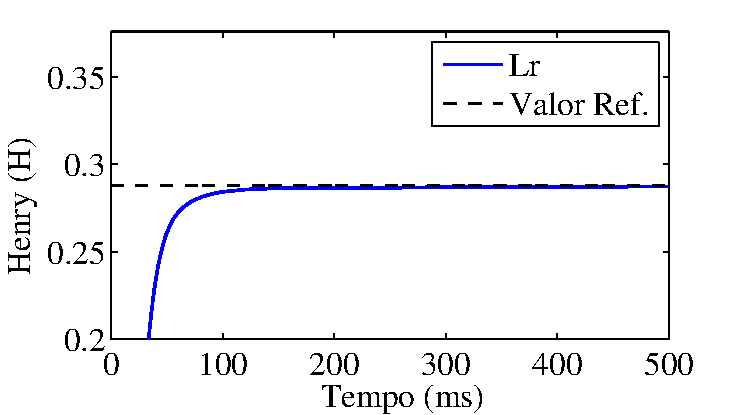
\includegraphics[width=.5\linewidth]{fig/grafico.pdf}
    \legend{Fonte: Elaborada pelo autor, 2020.}
\end{figure}

\begin{figure}[htb]
 \centering
  \begin{minipage}{0.45\textwidth}
    \caption{Gráfico 1}
    \label{fig:grafico1}
    \centering
    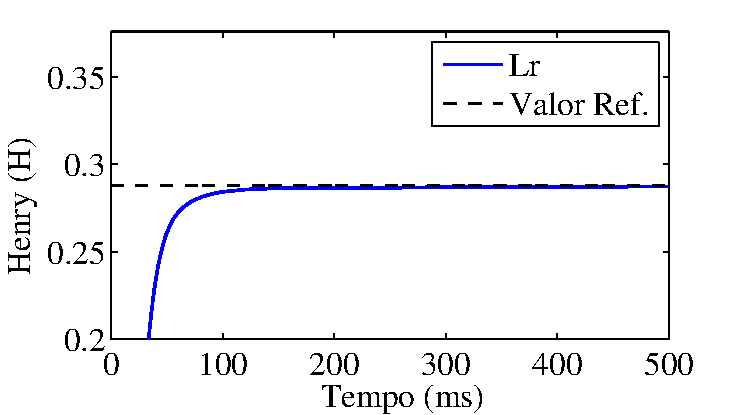
\includegraphics[scale=0.15]{fig/grafico.pdf}
    \legend{Fonte: \citeonline[p.~20]{exemplodelivro}.}
  \end{minipage}
  \hfill
  \begin{minipage}{0.45\textwidth}
    \caption{Gráfico 2}
    \label{fig:grafico2}
    \centering
    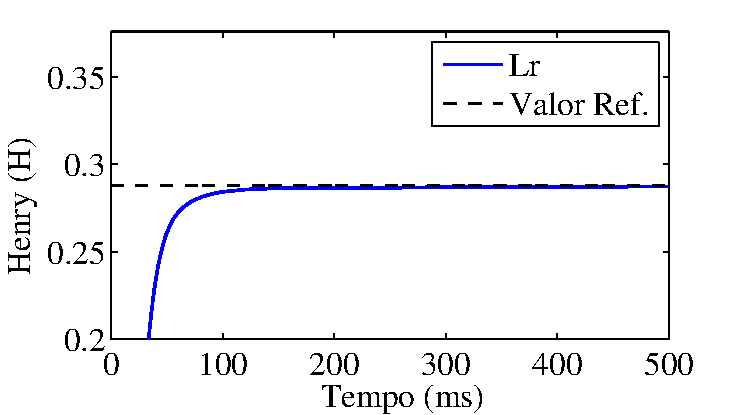
\includegraphics[scale=0.15]{fig/grafico.pdf}
    \legend{Fonte: \citeonline[p.~20]{exemplodelivro}.}
  \end{minipage}
\end{figure}

\section{Tabela}\label{texto:exemplo:tabela}

A \autoref{tab:exemplo} é um exemplo.

\begin{table}[htb]
    \caption{Tabela de exemplo}
    \label{tab:exemplo}
    \centering
    \ABNTEXfontereduzida
    \begin{tabular}{l|l}
        \hline
        \textbf{Indivíduo} & \textbf{Resultado} \\
        \hline
        A & 5 \\
        \hline
        B & 7 \\
        \hline
    \end{tabular}
    \legend{Fonte: \citeonline{exemplodelivro}.}
\end{table}

\section{Expressões matemáticas}\label{texto:exemplo:expressoesmatematicas}

Use o contexto \texttt{equation} para escrever
expressões matemáticas, conforme o exemplo da \autoref{eq:exemplo}.

\begin{equation}
    \label{eq:exemplo}
    \Delta s  = v \cdot t
\end{equation}

\section{Nota de rodapé}\label{texto:exemplo:notarodape}

Este texto possui uma nota de rodapé\footnote{Esta é uma nota de rodapé.}.

\section{Siglas}\label{texto:exemplo:siglas}

As siglas devem ser definidas no arquivo \texttt{pretexto/siglas.tex}, depois podem ser utilizadas com \ac{OV} para singular, ou \acp{OV} para plural. Na primeira vez o nome aparecerá por extenso, nas demais apenas a sigla.

Outros exemplo: \ac{SDN} e \ac{SGBD}.

Veja mais em: \url{https://www.ctan.org/pkg/acronym}.

\section{Seção secundária}\label{texto:exemplo:secao-secundaria}

Exemplo de seção secundária.

\subsection{Seção terciária}\label{texto:exemplo:secao-secundaria:secao-terciaria}

Exemplo de seção terciária.

\subsubsection{Seção quaternária}\label{texto:exemplo:secao-secundaria:secao-terciaria:secao-quaternaria}

Exemplo de seção quaternária.

\subsubsubsection{Seção quinária}\label{texto:exemplo:secao-secundaria:secao-terciaria:secao-quaternaria:secao-quinaria}

Exemplo de seção quinária.

E qualquer seção pode ser referenciada com nestes exemplos: \autoref{texto:exemplo} e \autoref{texto:exemplo:secao-secundaria:secao-terciaria:secao-quaternaria:secao-quinaria}.

\section{Enumeração}\label{texto:exemplo:enumeracao}

\begin{alineas}
    \item Itens enumerados;
    \item Sub-itens:
    \begin{alineas}
        \item 1;
        \item 2.
    \end{alineas}
    \item O último termina com ponto.
\end{alineas}

    \chapter{Introdução}\label{texto:introducao}

Texto...

    \chapter{Conclusão}\label{texto:conclusao}

Texto...



    % Elementos Pós-textuais

    \postextual

    \bibliography{referencias}

    % Apêndices
    \begin{apendicesenv}
        \chapter{Exemplo de apêndice}\label{apendice:exemplo}

Texto...

    \end{apendicesenv}

    % Anexos
    \begin{anexosenv}
        \chapter{Exemplo de anexo}\label{anexo:exemplo}

Texto...

    \end{anexosenv}
\end{document}
